%%%%%%%%%%%%%%%%%%%%%%%%%%%%%%%%%%%%%%%%%%%%%%
%                insertmeeting
% 1) Title (something creative & funny?)
% 2) Date (MM/DD/YYYY)
% 3) Location (ex. Hagerty High School)
% 4) People/Committees Present 
% 5) Picture 
% 6) Start Time & Stop Time (ex. 12:30AM to 4:30PM)
%%%%%%%%%%%%%%%%%%%%%%%%%%%%%%%%%%%%%%%%%%%%%%
\insertmeeting 
	{Cool Carbon} 
	{02/13/22} 
	{Hagerty High School}
	{James, Jensen, Samantha, Anouska, Annika, Clayton, Falon, Nathan, Ritam}
	{Images/RobotPics/robot.jpg}
	{2:30 - 4:30}
	
\hhscommittee{Software}
\noindent\hfil\rule{\textwidth}{.4pt}\hfil
\subsubsection*{Goals}
\begin{itemize}
    \item Get finished carbon fiber side from vacuum bag
	\item Remove carbon fiber from mold
	\item Paint the outside of both sides with epoxy

\end{itemize} 

\noindent\hfil\rule{\textwidth}{.4pt}\hfil

\subsubsection*{Accomplishments}
When the meeting started, we were quick to go over and grab the carbon fiber sides which our mentor had brought over from UCF. There was one problem though: the mold and carbon fiber were still stuck down to the glass plate. Before trying to remove it though, we took off the peel-ply layer to get a better look at the new side and how it was stuck to the glass (Figure \ref{fig:021322_1}). It appeared that we made our carbon fiber sheets too big, causing them to stick to the glass. We tried fruitlessly to pry the carbon fiber off. When this didn’t work, we knew we would have to cut it off of the glass plate with a dremel. Because carbon fiber dust can be dangerous to breathe in, we had to be very careful while cutting it. To keep ourselves safe, we wore masks while cutting (which we were already wearing because of covid) and used a diamond grit bit for the dremel, which cuts through materials faster and cleaner than other bits, meaning it creates less dust. As a final precaution, we decided to cut the carbon fiber under flowing water which will catch the dust. Although these precautions are more than may have been needed, we would rather be safe than sorry, which is why we were extra careful. Using the dremel, we cut through all of the extra carbon fiber that kept the mold stuck to the glass plate. After getting the parts off the glass, the carbon fiber was still stuck very firmly to the mold. Remembering what we did with the other mold, we got popsicle sticks and started pressing them into gaps between the mold and the carbon fiber to slowly push the carbon fiber off of the mold (Figure \ref{fig:021322_2}). Although it took more popsicle sticks than last time, (probably because of the odd shape of the second side which added more friction between the mold and the carbon fiber) we were still able to successfully separate the two parts (Figure \ref{fig:021322_3}). To finish off the meeting, we decided to paint the duller colored outsides of the carbon fiber with a layer of epoxy to give it the classic carbon fiber look (Figure \ref{fig:021322_4}). 

\begin{figure}[ht]
\centering
\begin{minipage}[b]{.48\textwidth}
  \centering
  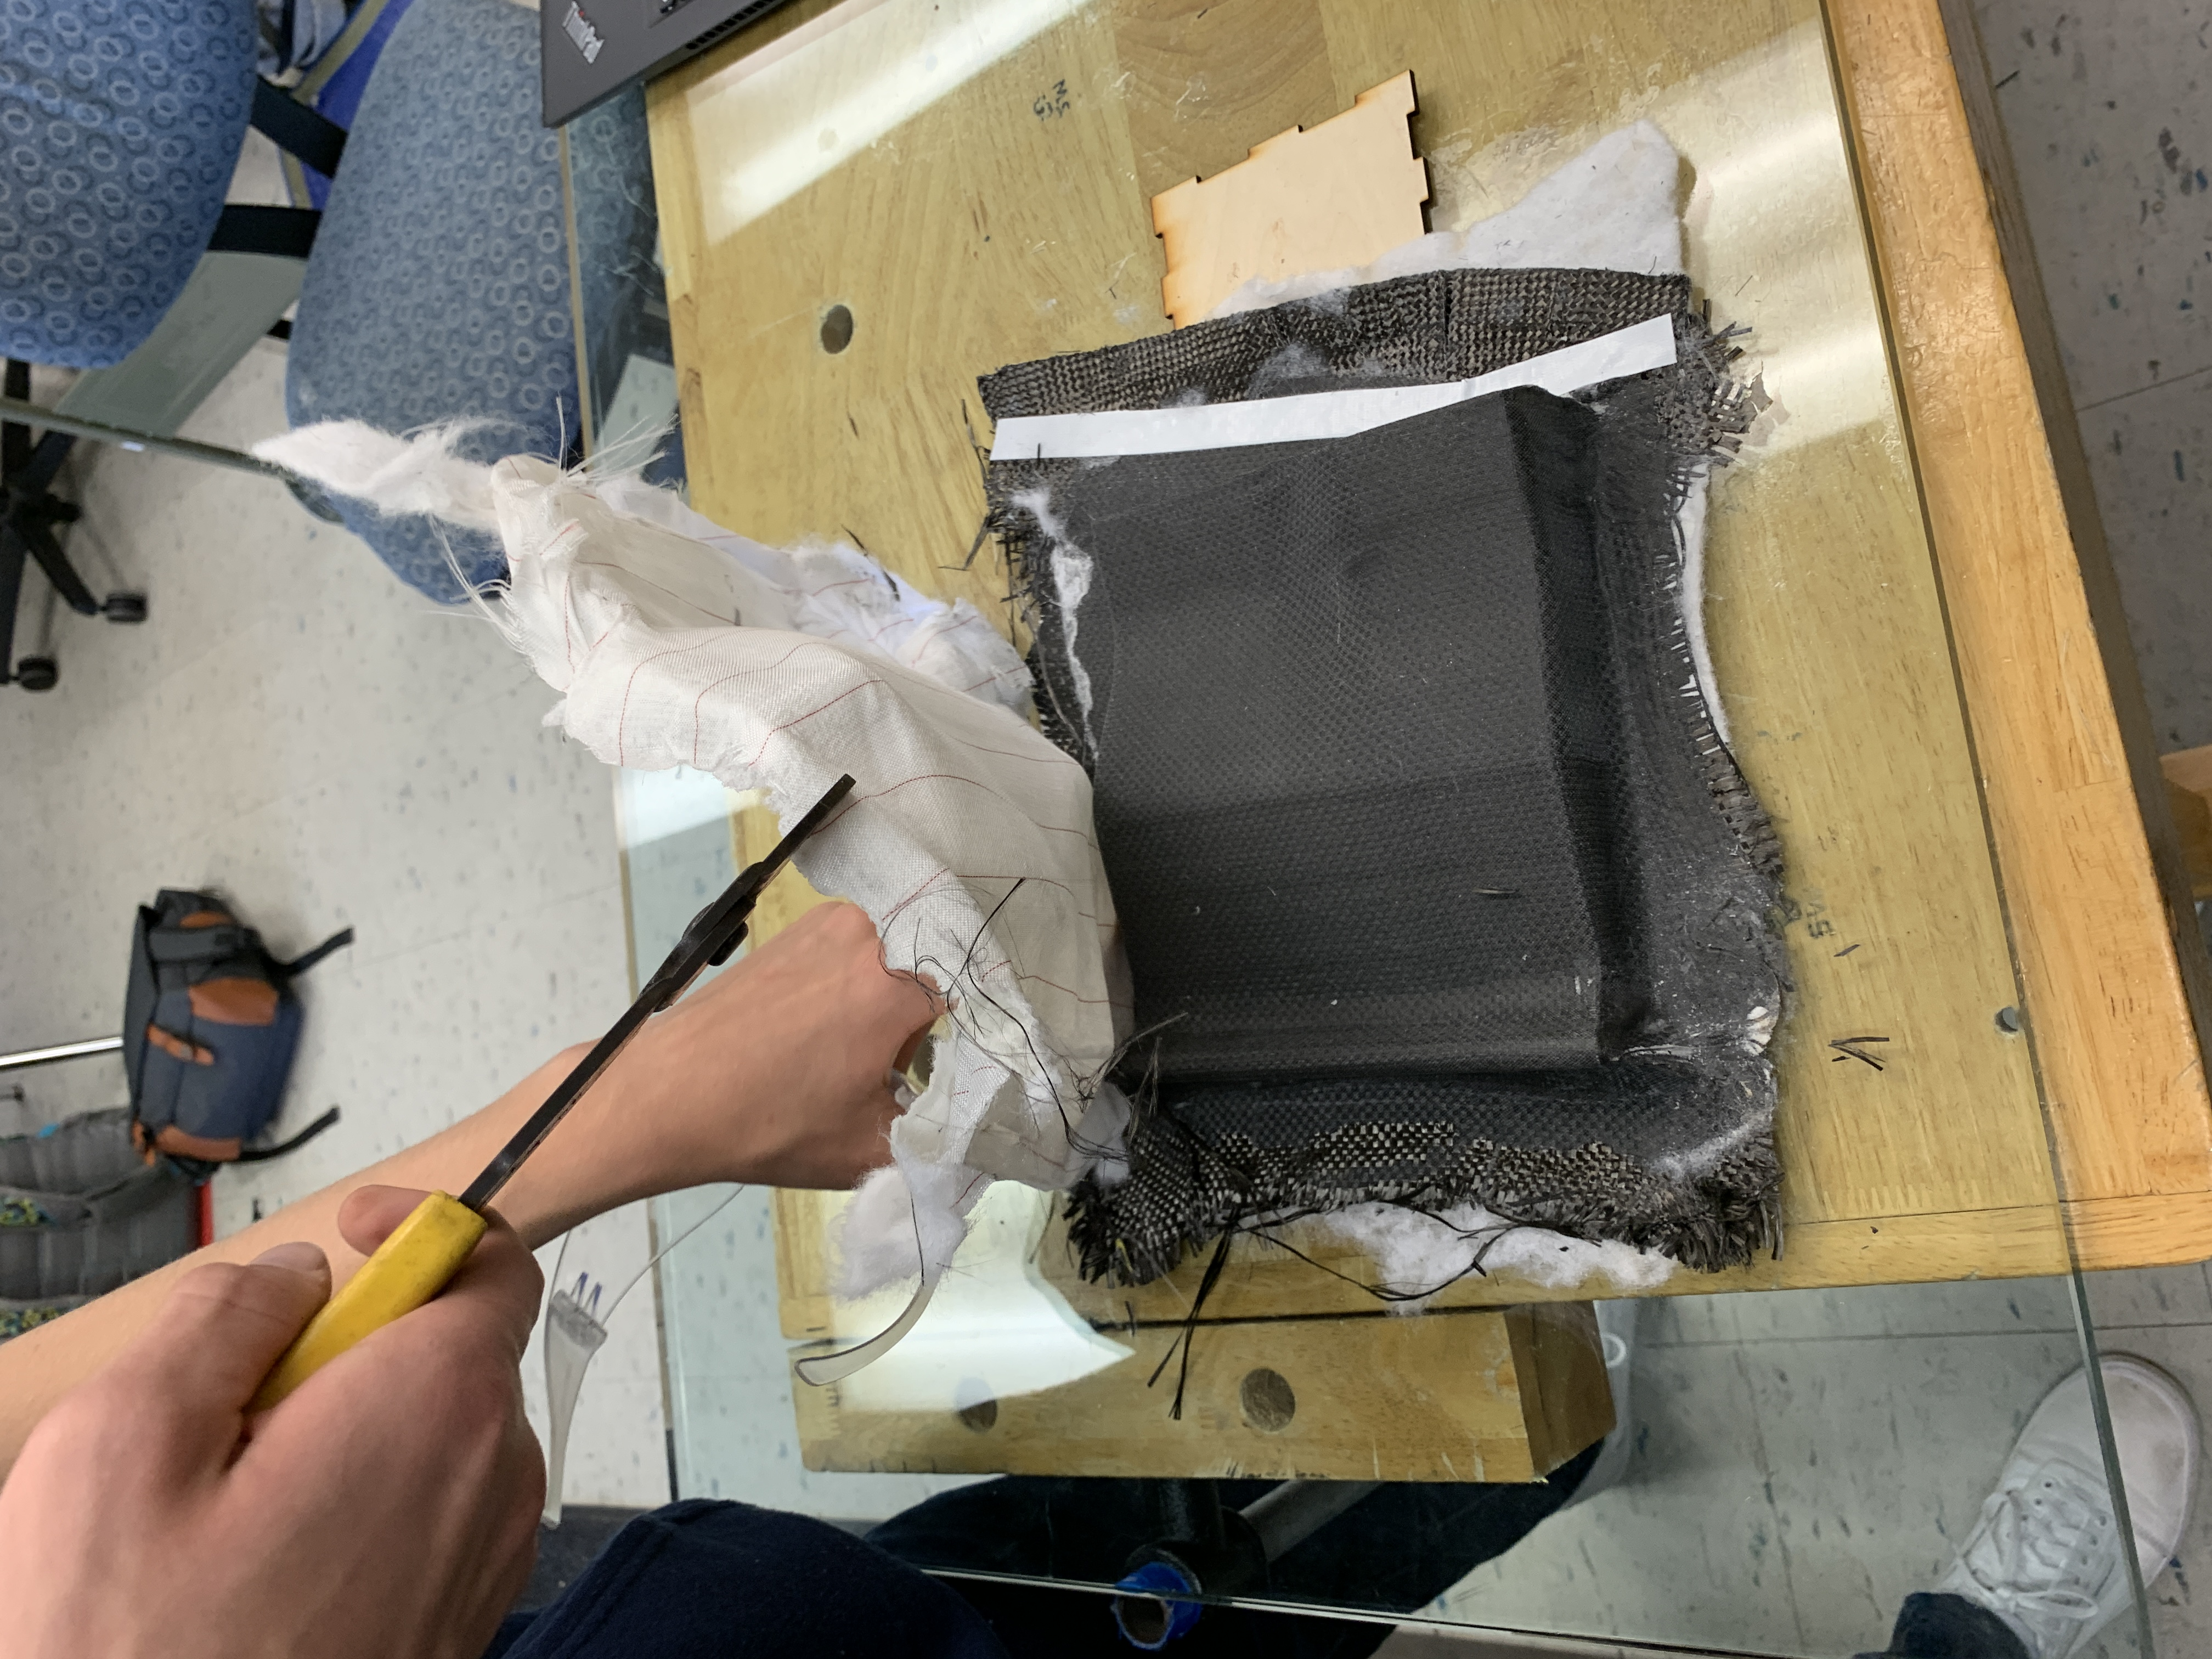
\includegraphics[width=0.95\textwidth]{Meetings/February/02-13-22/2-12-22_Hardware_Figure1 - Nathan Forrer.JPG}
  \caption{Sticking to the glass}
  \label{fig:021322_1}
\end{minipage}%
\hfill%
\begin{minipage}[b]{.48\textwidth}
  \centering
  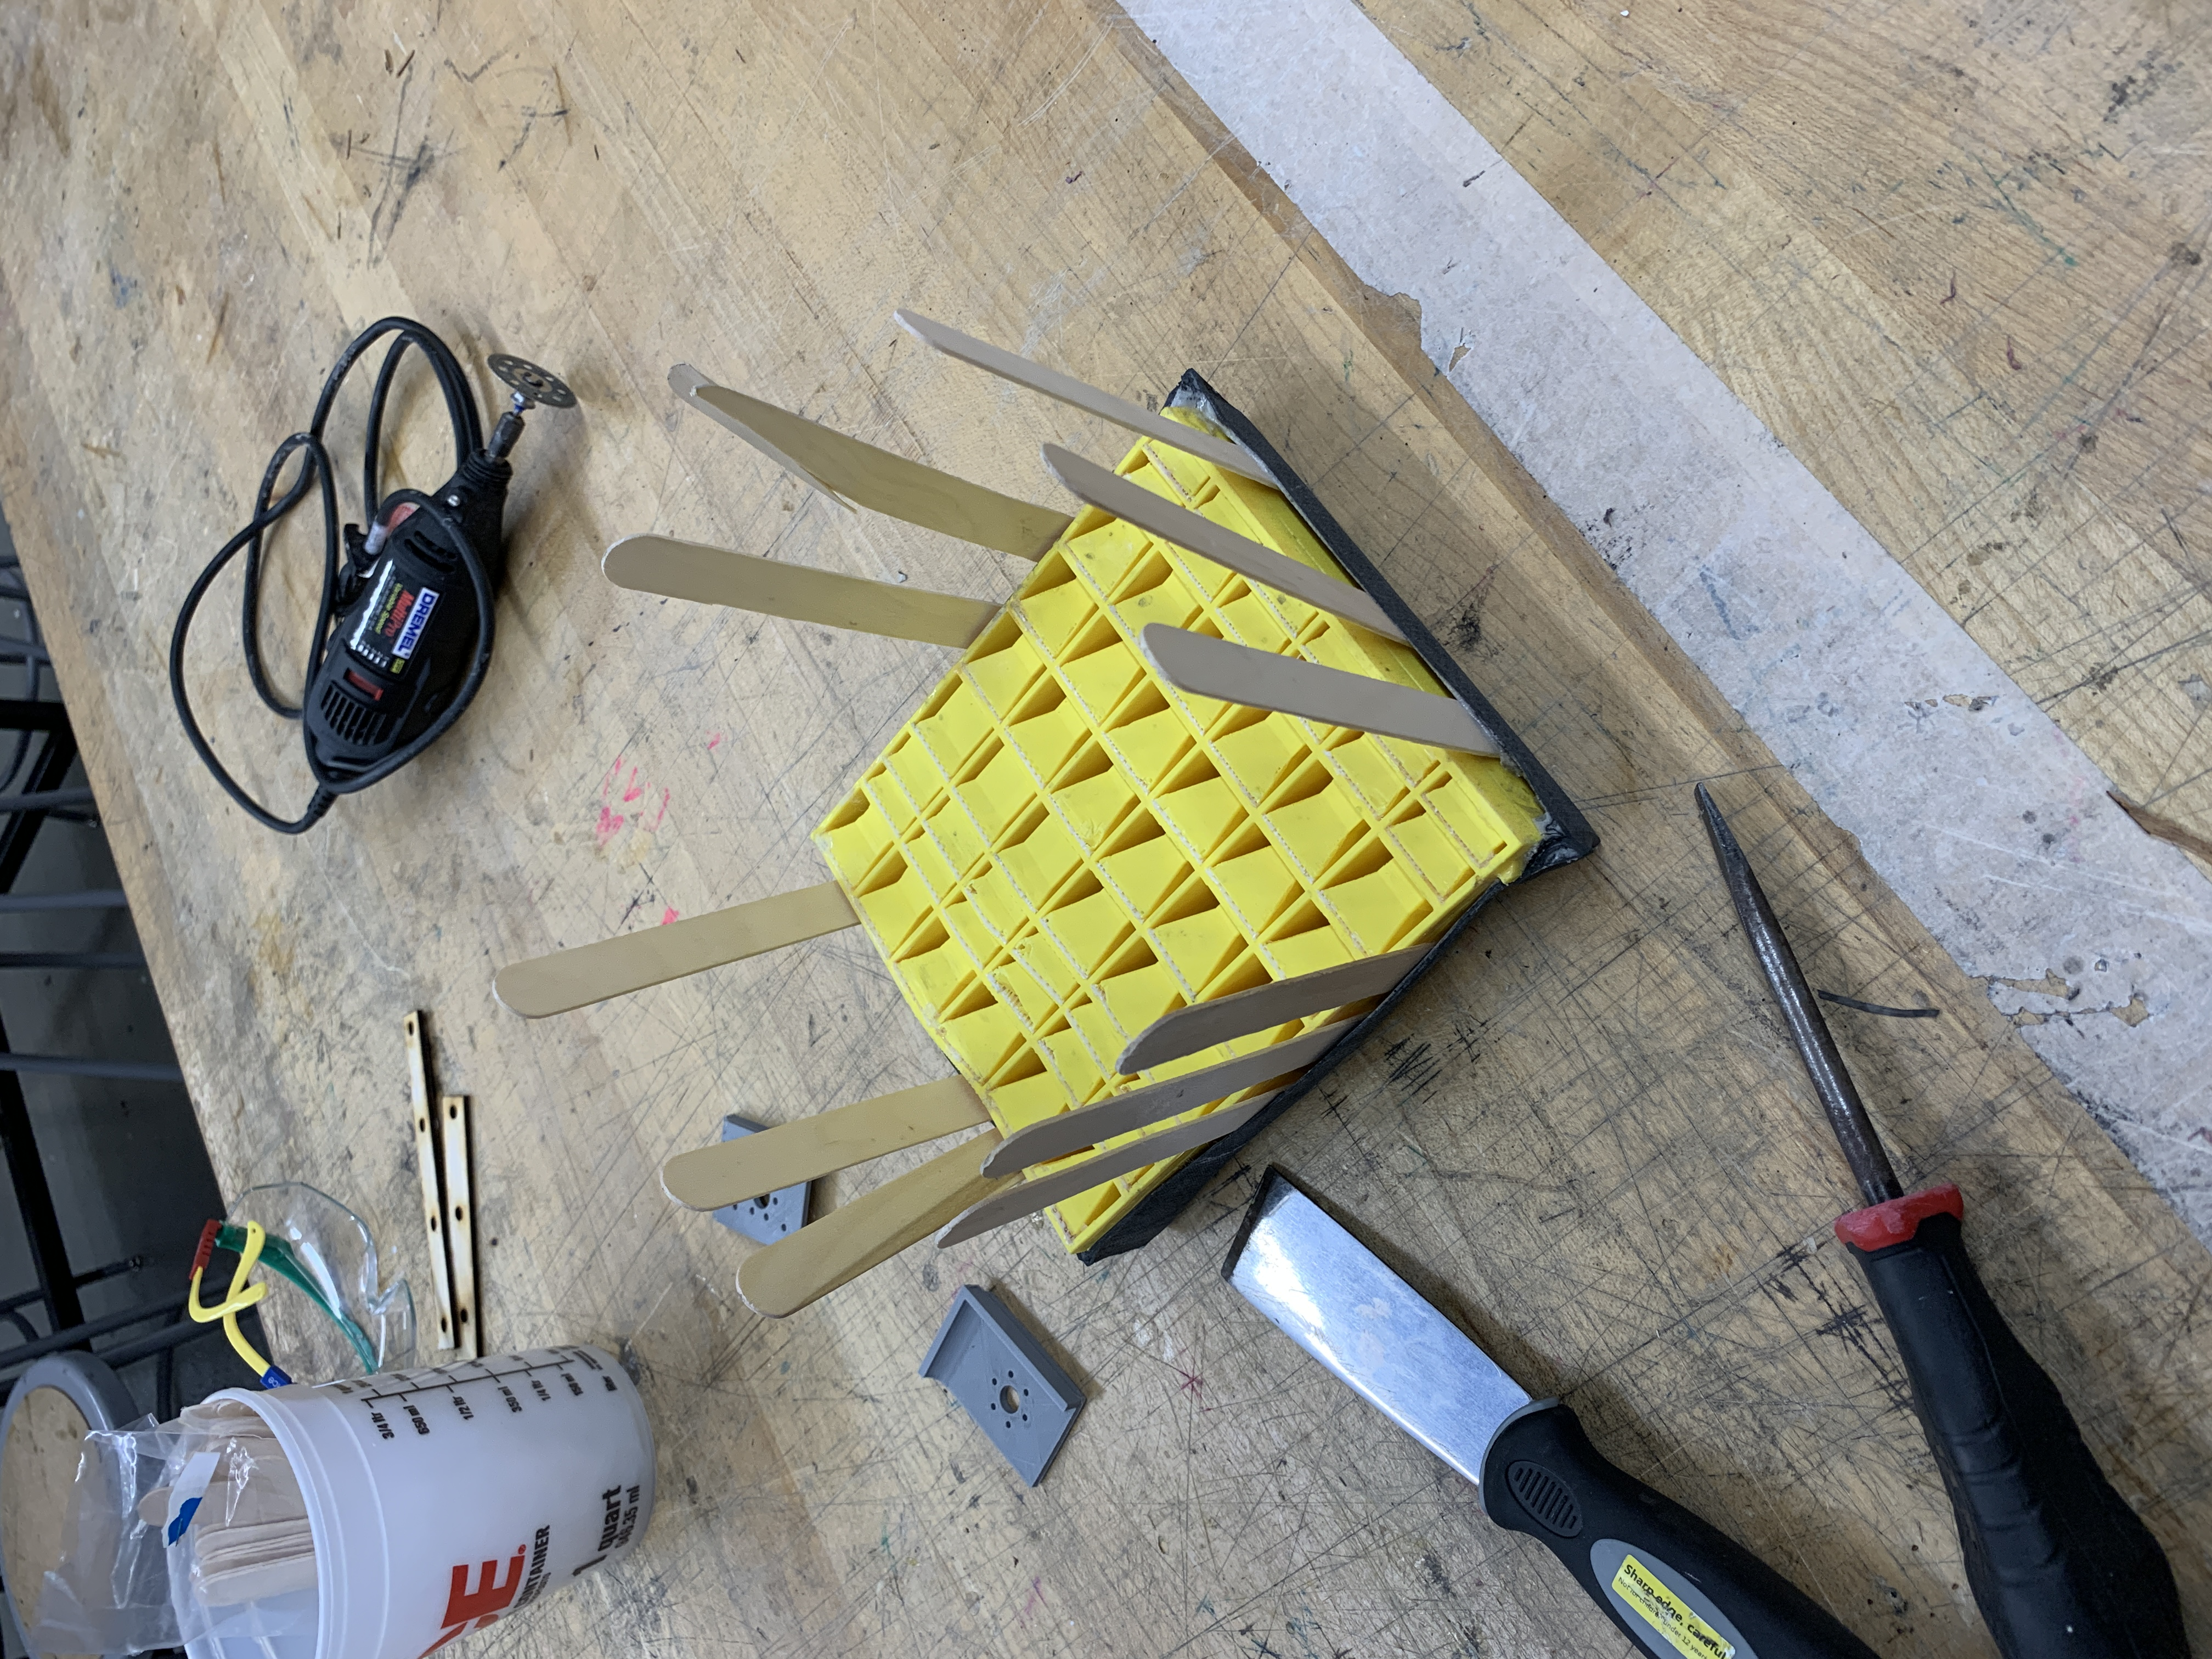
\includegraphics[width=0.95\textwidth]{Meetings/February/02-13-22/2-12-22_Hardware_Figure2 - Nathan Forrer.JPG}
  \caption{Pressing in popsicle sticks}
  \label{fig:021322_2}
\end{minipage}
\end{figure}

\begin{figure}[ht]
\centering
\begin{minipage}[b]{.48\textwidth}
  \centering
  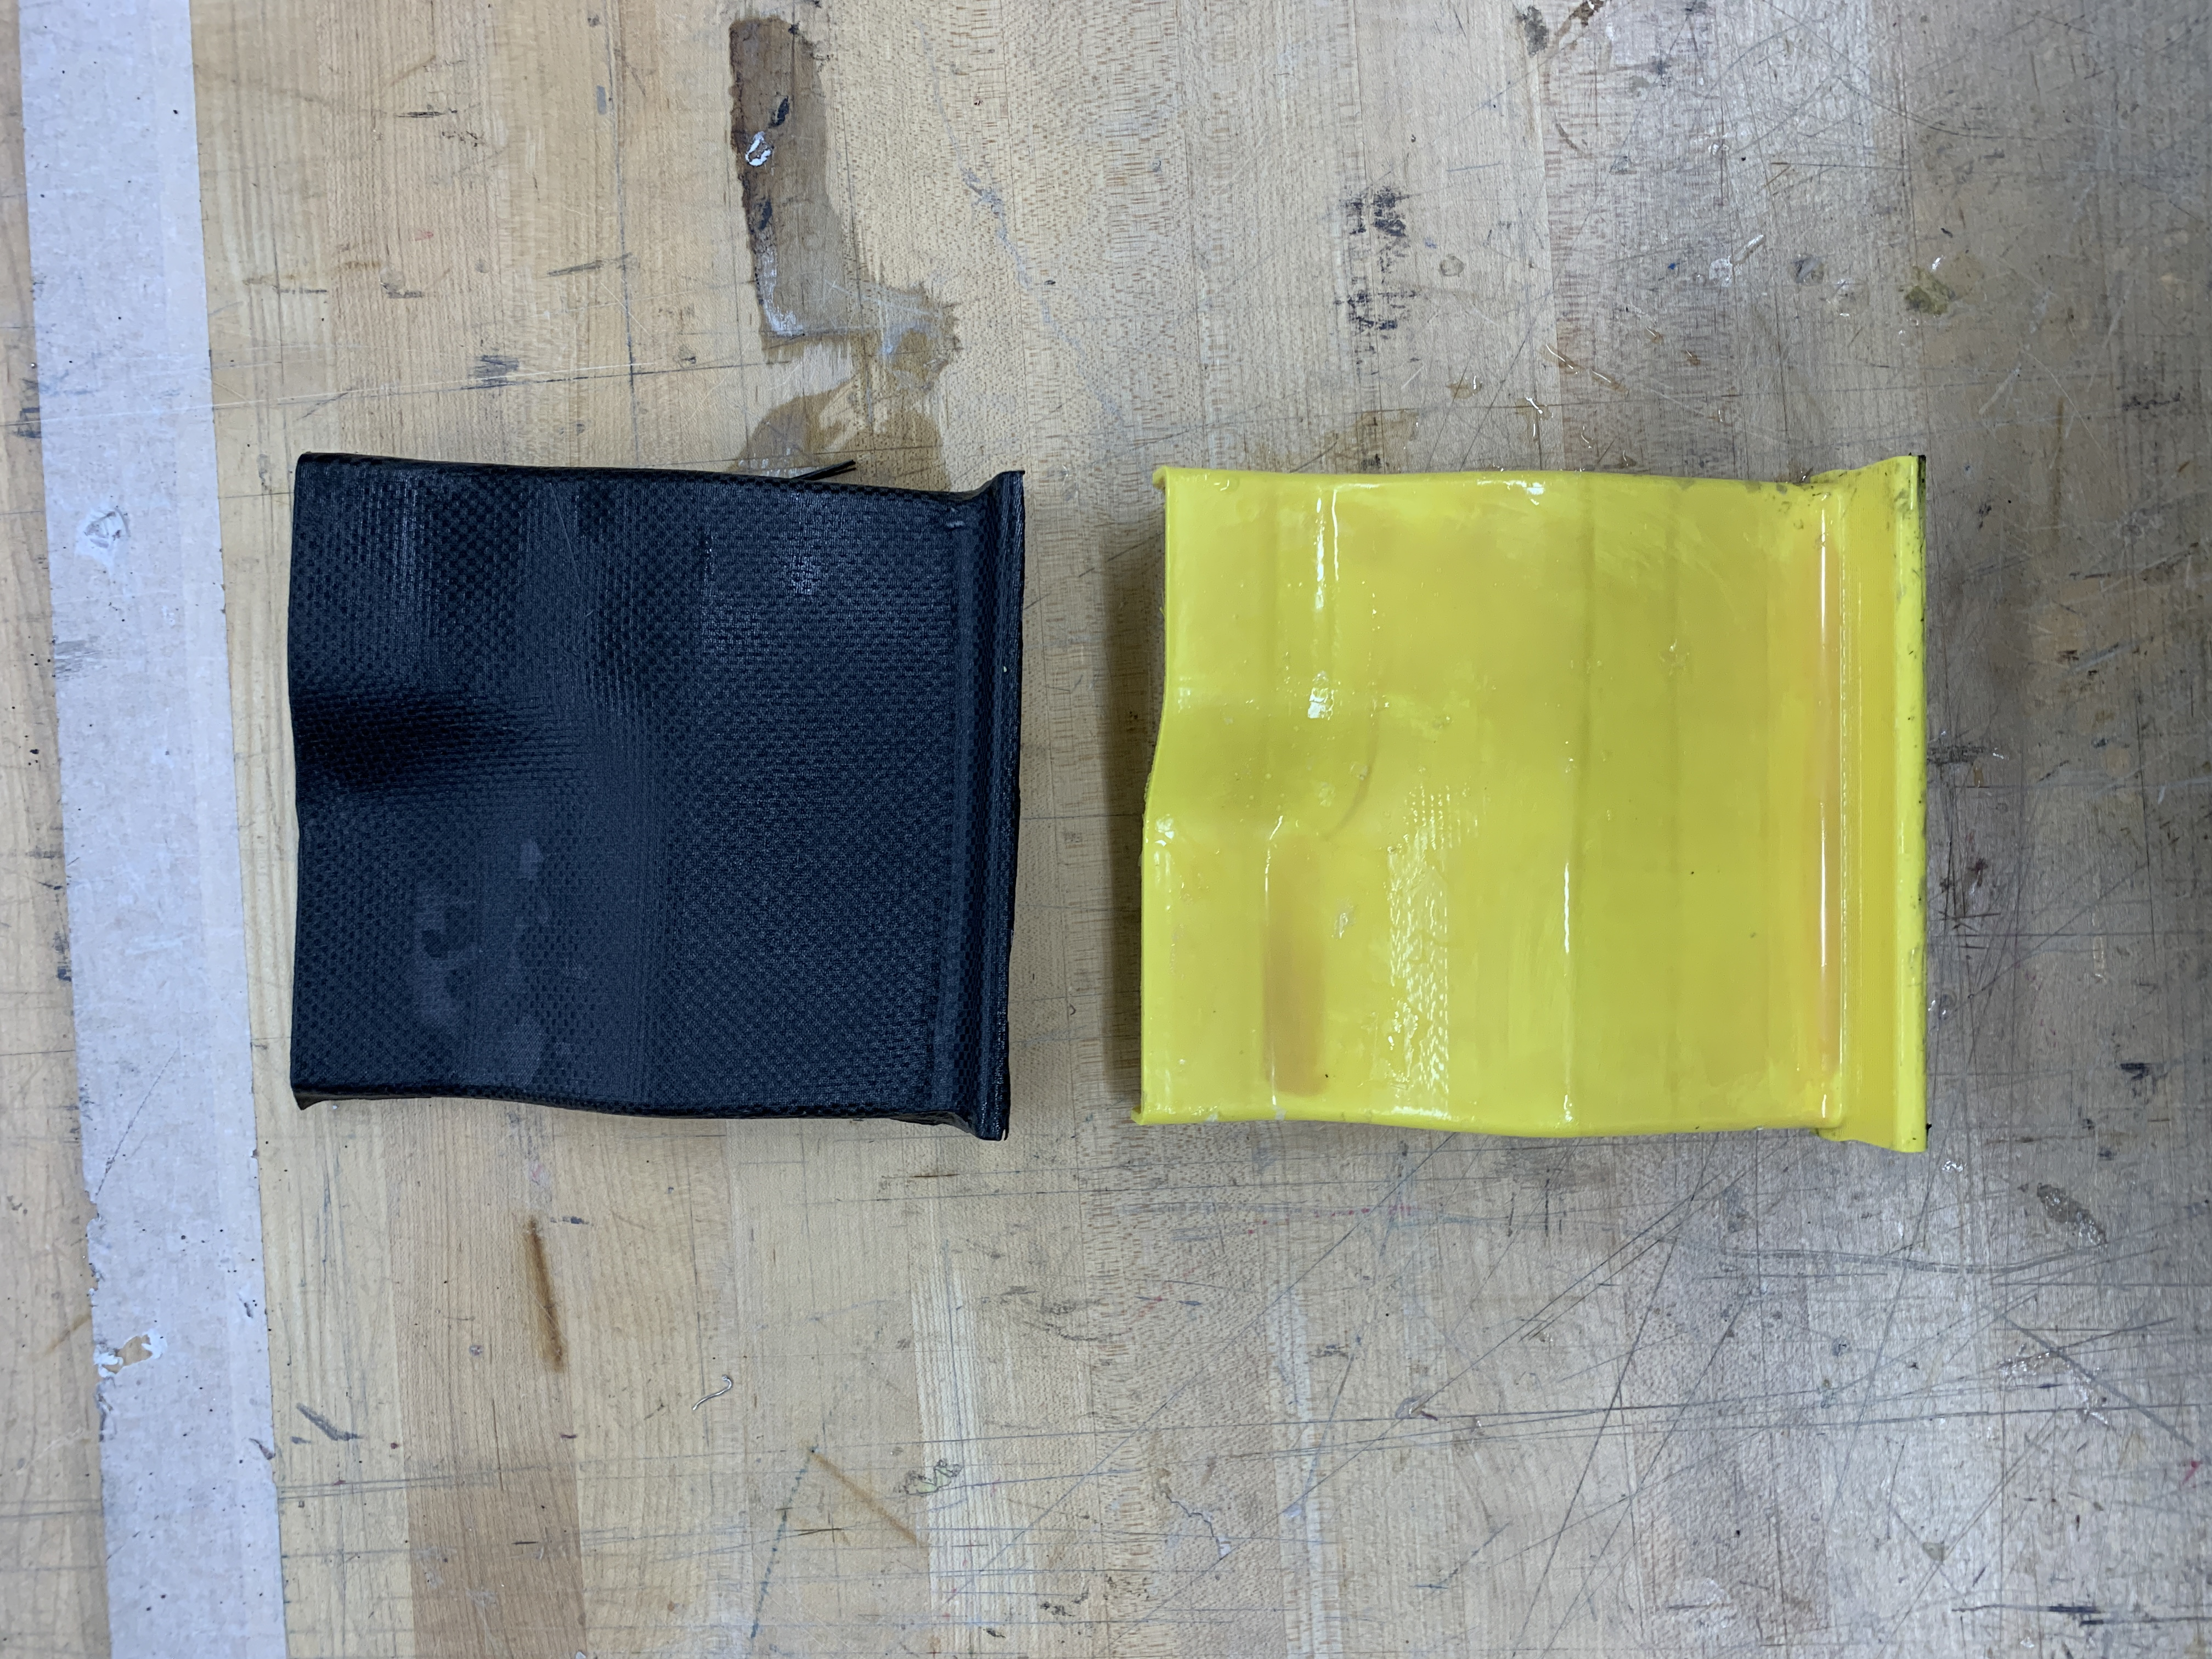
\includegraphics[width=0.95\textwidth]{Meetings/February/02-13-22/2-12-22_Hardware_Figure3 - Nathan Forrer.JPG}
  \caption{Separating the two parts}
  \label{fig:021322_3}
\end{minipage}%
\hfill%
\begin{minipage}[b]{.48\textwidth}
  \centering
  \includegraphics[width=0.95\textwidth]{Meetings/February/02-13-22/2-12-22_Hardware_Figure4 - Nathan Forrer.JPG}
  \caption{Painting with epoxy}
  \label{fig:021322_4}
\end{minipage}
\end{figure}


\whatsnext{
\begin{itemize}
    \item Start drilling holes in carbon fiber
	\item Assemble carbon fiber sides

\end{itemize} 
}

